\chapter{Attachments} \label{chap:attachments}

% ~~~~~~~~~~~~~~~~~~~~~~~~~~~~~~~~~~~~~~~~~~~~~~~~~~~~~~~~~~~~~~~~~~~~~~~~~~~~~~~~~~~~~~~~~~~~~~~~~~~~~~~~~~~
\section{Algorithms, Functions, and Procedures} \label{sec:attachments/algorithms-functions-procedures}


\begin{alg}{Function}{GranularResourceLoad}{$k$, $\Instance$, $\Schedule$, $PC$} \label{alg:granular-resource-load}
\State $L : \intinterval{1}{PC} \to \Nzero$
       \Comment Period load function
\For {$j \in \JobsOnResource{k}$}
    \State $i_l \gets \lfloor \jobstart{j} / \algGranularity \rfloor$,
           \Comment{First overlapping period}
    \State $i_h \gets \lfloor \jobend{j} / \algGranularity \rfloor$
           \Comment{Last overlapping period}
    \If {$i_l = i_h$}
        \Comment{If the job overlaps with a single period...}
        \State $L(i_l) \gets L(i_l) + \duration{j} \consumption{j}{k}$
    \Else
        \Comment{...the job overlaps with multiple periods}
        \State $L(i_l) \gets L(i_l) + (\algGranularity (i_l + 1) - \jobstart{j}) \cdot \consumption{j}{k}$
        \For {$i \in \intinterval{i_l+1}{i_h-1}$}
            \State $L(i) \gets L(i) + \algGranularity \cdot \consumption{j}{k}$
        \EndFor
        \State $L(i_h) \gets L(i_h) + (\jobend{j} - \algGranularity (i_h - 1)) \cdot c$
    \EndIf
\EndFor
\State \Return $L$
\end{alg}


\begin{alg}{Function}{IncreaseGranularPeriodCapacity}{$i$, $\capacityf{k}$, $\algGranularity$, $\algImprovement$} \label{alg:increase-granular-period-capacity}
\State $t_l \gets 1+ (i-1)\algGranularity$
       \Comment First time period covered
\State $t_h \gets i \algGranularity$
       \Comment Last time period covered
\For{$t \in \intinterval{t_l}{t_h}$}
    \State $\capacity{k}{t} \gets \capacity{k}{t} + \algImprovement$
\EndFor
\State \Return $\capacity{k}{t}$
\end{alg}


\begin{alg}{Function}{ReduceCapacityChanges}{$\Instance$, $\Schedule$, $\capacityf{1}^\text{orig}$, \dots, $\capacityf{m}^\text{orig}$} \label{alg:reduce-capacity-changes}
\State $\capacityf{1}^\prime, \dots, \capacityf{m}^\prime: \intinterval{1}{\horizon} \to \Nzero$
       \Comment Reduced capacity functions
\For {$k \in \Resources$}
    \State $L \gets $ \Callref{ResourceLoad}{$k$, $\Instance$, $\Schedule$}{alg:resource-load}
    \For {$t \in \intinterval{1}{\horizon}$}
        \State $\capacity{k}{t}^\prime \gets \max(\capacity{k}{t}^{\text{orig}}, L(t))$
    \EndFor
\EndFor
\State \Return $\capacityf{1}^\prime, \dots, \capacityf{m}^\prime$
\end{alg}


\begin{alg}{Function}{ResourceLoad}{$k$, $\Instance$, $\Schedule$} \label{alg:resource-load}
\State $L : \intinterval{1}{\horizon} \to \Nzero$
\For {$t \in \intinterval{1}{\horizon}$}
    \State $L(t) \gets \sum_{j \in \JobsOnResourceInTimePeriod{k}{t}} \consumption{j}{k}$
        \Comment $\JobsOnResourceInTimePeriod{k}{t}$ with respect to given schedule $\Schedule$
\EndFor
\State \Return $L$
\end{alg}


\begin{alg}{Function}{FindAdditionsAndMigrations}{$\Instance$, $\Schedule$} \label{alg:find-additions-and-migrations}
\State $\Migrations \gets \emptyset$
\For {$(\forall k \in \Resources)$} $L_k \gets$ \Callref{ResourceLoad}{$k$, $\Instance$, $\Schedule$}{alg:resource-load} \EndFor
\For {$(\forall k \in \Resources)$} $\capacityf{k}^\oplus \gets \capacityf{k} - L_k$ \Comment Capacity surpluses \EndFor
\State REQ $\gets$ set of all additional non-shift capacities

\For {$(k, s, e, c) \in$ REQ}
    \While {$c > 0$}
        \State $c_1, \dots, c_m \gets$ maximal continuous surpluses overlapping $\intinterval{s}{e}$
        \State $k_\text{from} \gets \argmax_k{c_k}$
        \If {$c_{k_\text{from}} = 0$} \Comment If no further migrations are possible
            \State \textbf{break} \Comment Remaining $c$ will be fulfilled by capacity additions
        \EndIf
        \State $c_\text{mig} \gets \min(c, c_{k_\text{from}})$
        \State Reduce surplus $\capacityf{k_{\text{from}}}^\oplus$ by $c_{\text{mig}}$ during time periods $\intinterval{s}{e}$
        \State $\Migrations \gets \Migrations \cup \{ \migration{k_\text{from}}{k}{s}{e}{c_{\text{mig}}} \}$
    \EndWhile
\EndFor

\State $\Additions \gets \left\{ \addition{k}{s}{e}{c} \in \text{ REQ} : c > 0 \right\}$

\State \Return $\Additions$, $\Migrations$
\end{alg}


\begin{alg}{Function}{ModifyResourceCapacities}{$\Instance$, $\chi_1$, \dots, $\chi_c$} \label{alg:modify-resource-capacities}
\State $\capacityf{1}^*, \dots, \capacityf{m}^* \gets \capacityf{1}, \dots, \capacityf{m}$
    \Comment Copy the original capacity functions
\For {$(j, s, e) \in \{ \chi_1, \dots, \chi_c \}$}
    \For {$k \in \Resources : \consumption{j}{k} > 0 $}
        \For {$t \in \intinterval{s}{e-1}$}
            \State $\capacity{k}{t}^* \gets \capacity{k}{t}^* + \consumption{j}{k}$
        \EndFor
    \EndFor
\EndFor
\State \Return $\capacityf{1}^*, \ldots, \capacityf{m}^*$
\end{alg}


\begin{alg}{Function}{ComputeSuffixRelaxedSchedule}{$\Instance$, $\Schedule$, $t$} \label{alg:suffix-relaxed-schedule}
\State $T \gets $ Topological ordering of $\Jobs$ on the precedence graph $G$
\For {$j \in T$}
    \If {$\jobstart{j} \leq t$}
        \State $\relaxedjobstart{t}{j} \gets \jobstart{j}$
    \Else
        \State $\relaxedjobstart{t}{j} \gets \max\left\{\relaxedjobstart{t}{i} + \duration{i} : \precedence{i}{j} \in \Precedences \right\}$
    \EndIf
\EndFor
\State \Return $\relaxedSchedule{t}$
\end{alg}

\newpage
\begin{alg}{Function}{ComputeLeftShiftClosure}{$\Instance$, $\Schedule$, $j$} \label{alg:left-shift-closure}
\State $\closure{j} \gets \emptyset$
\State $Q \gets \{j\}$ \Comment Queue of jobs to process
\While {$Q \text{ not empty}$}
    \State $i \gets$ pop $Q$
    \State $\closure{j} \gets \closure{j} \cup \{ i \}$
    \State $Q \gets Q \cup \{ p : \precedence{p}{i}, \jobend{p} = \jobstart{i}\}$
        \Comment Precedence predecessors
    \State $Q \gets Q \cup \bigcup_{k: \consumption{j}{k} > 0}\{ p \in \JobsOnResource{k} : \jobend{p} = \jobstart{i} \}$
        \Comment Resource predecessors
    \For {$k \in \Resources, \consumption{j}{k} > 0, \capacity{k}{\jobstart{i}-1} = 0$}
        \Comment Resource-pause predecessors
        \State $\mathrm{ps}_k(\jobstart{i}) \gets \max\{t^\prime \in \intinterval{1}{\jobstart{i}-1} : \capacity{k}{t^\prime} > 0\}$
        \State $Q \gets Q \cup \{ p \in \JobsOnResource{k} : \mathrm{ps}_k(\jobstart{i}) - \duration{i} \leq \jobend{p} \leq \mathrm{ps}_k(\jobstart{i}) \}$
    \EndFor
\EndWhile
\State \Return $\closure{j}$
\Statex
\Note  We assume, that when the value of $\mathrm{ps}_k(\jobstart{i})$ is undefined,
       the following set of predecessors
\Notec is trivially empty and we continue with a different resource.
\end{alg}

% ~~~~~~~~~~~~~~~~~~~~~~~~~~~~~~~~~~~~~~~~~~~~~~~~~~~~~~~~~~~~~~~~~~~~~~~~~~~~~~~~~~~~~~~~~~~~~~~~~~~~~~~~~~~
\section{Documentation} \label{sec:attachments/documentation}

\todo{Dokumentace}

\begin{small}
\begin{verbatim}
usage: experiments.py [--aggregate] [--scale] [--save_plots]
                      [--addition ADDITION] [--migration MIGRATION]
                                                                                                               
options:                                                                                                       
  --aggregate            Determines whether to aggregate
                         instances by type                                      
  --scale                Determines whether to scale
                         evaluations KPIs                                           
  --save_plots           Determines whether to save plots to files                                              
  --addition ADDITION    Cost of capacity addition                                                              
  --migration MIGRATION  Cost of capacity migration
\end{verbatim}
\end{small}

% ~~~~~~~~~~~~~~~~~~~~~~~~~~~~~~~~~~~~~~~~~~~~~~~~~~~~~~~~~~~~~~~~~~~~~~~~~~~~~~~~~~~~~~~~~~~~~~~~~~~~~~~~~~~
\section{Full instance plots} \label{sec:attachments/full-instance-plots}

\begin{figure}[p]
    \centering
    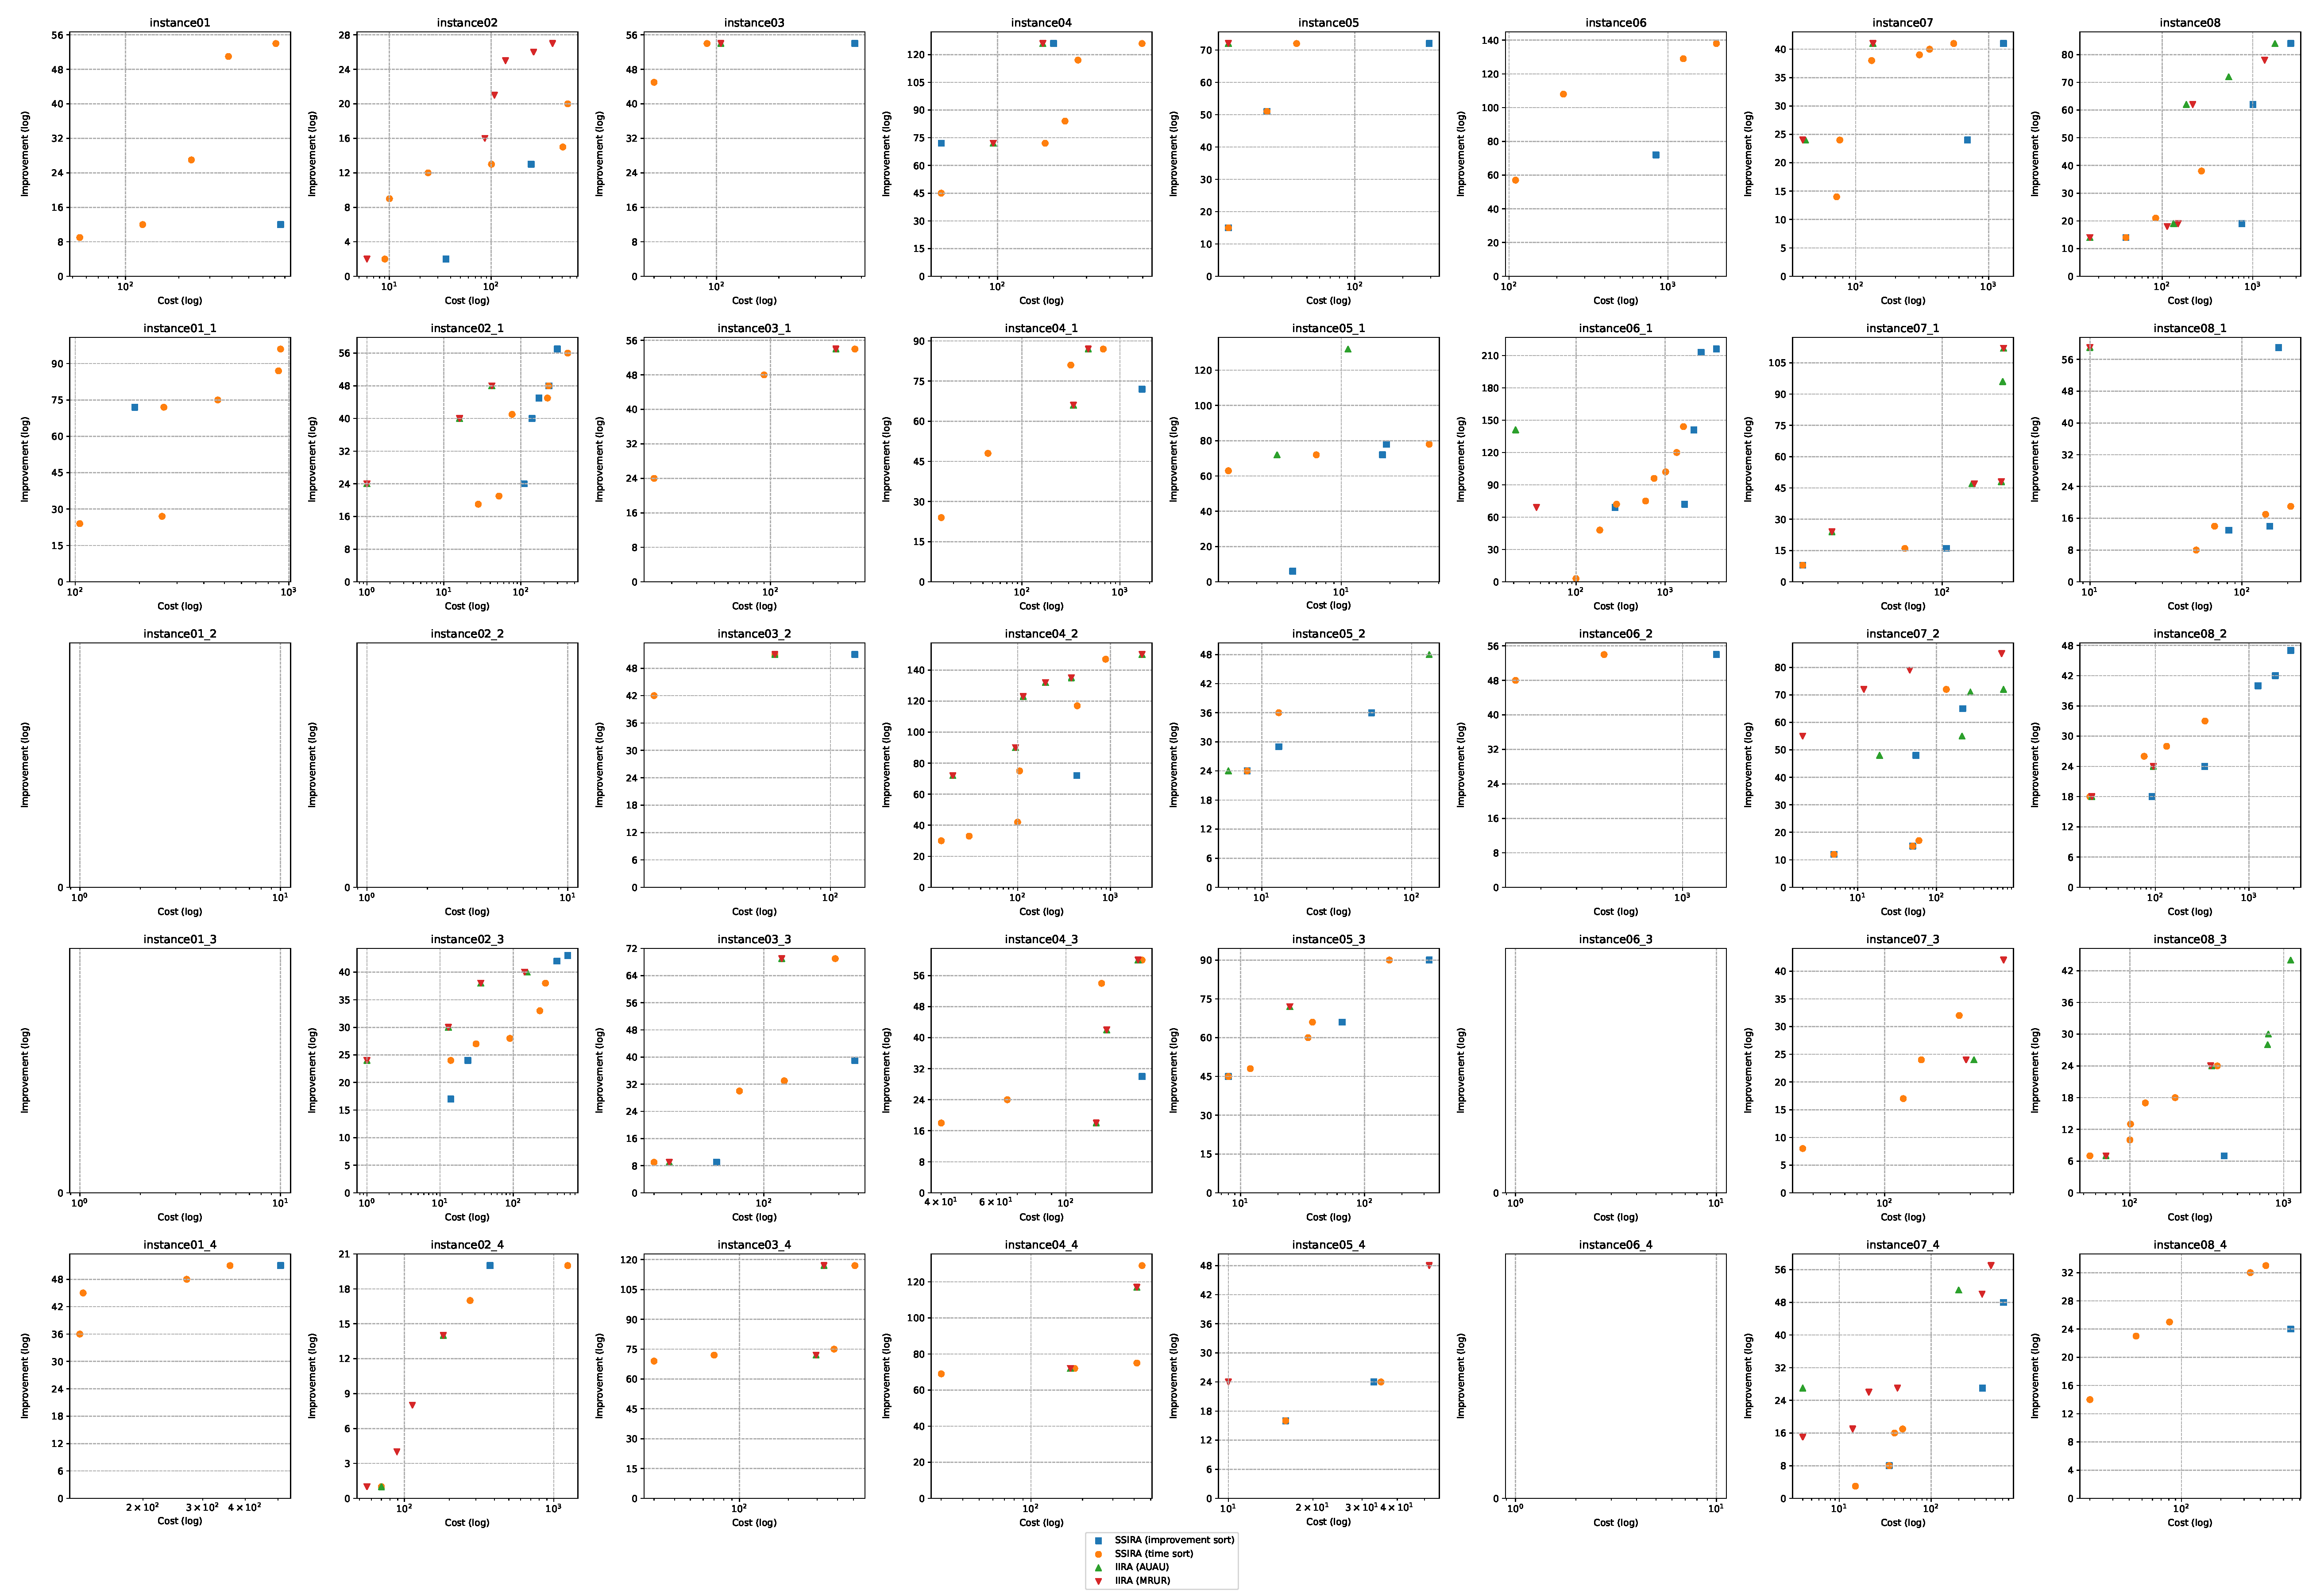
\includegraphics[angle=270, width=\textwidth]{img/exp_cost_improv.pdf}
    \caption{
        Capacity changes cost (x-axis) to achieved 
        improvement (y-axis) for every experiment instance.
        }
    \label{fig:exp-full/cost-improv}
\end{figure}

\begin{figure}[p]
    \centering
    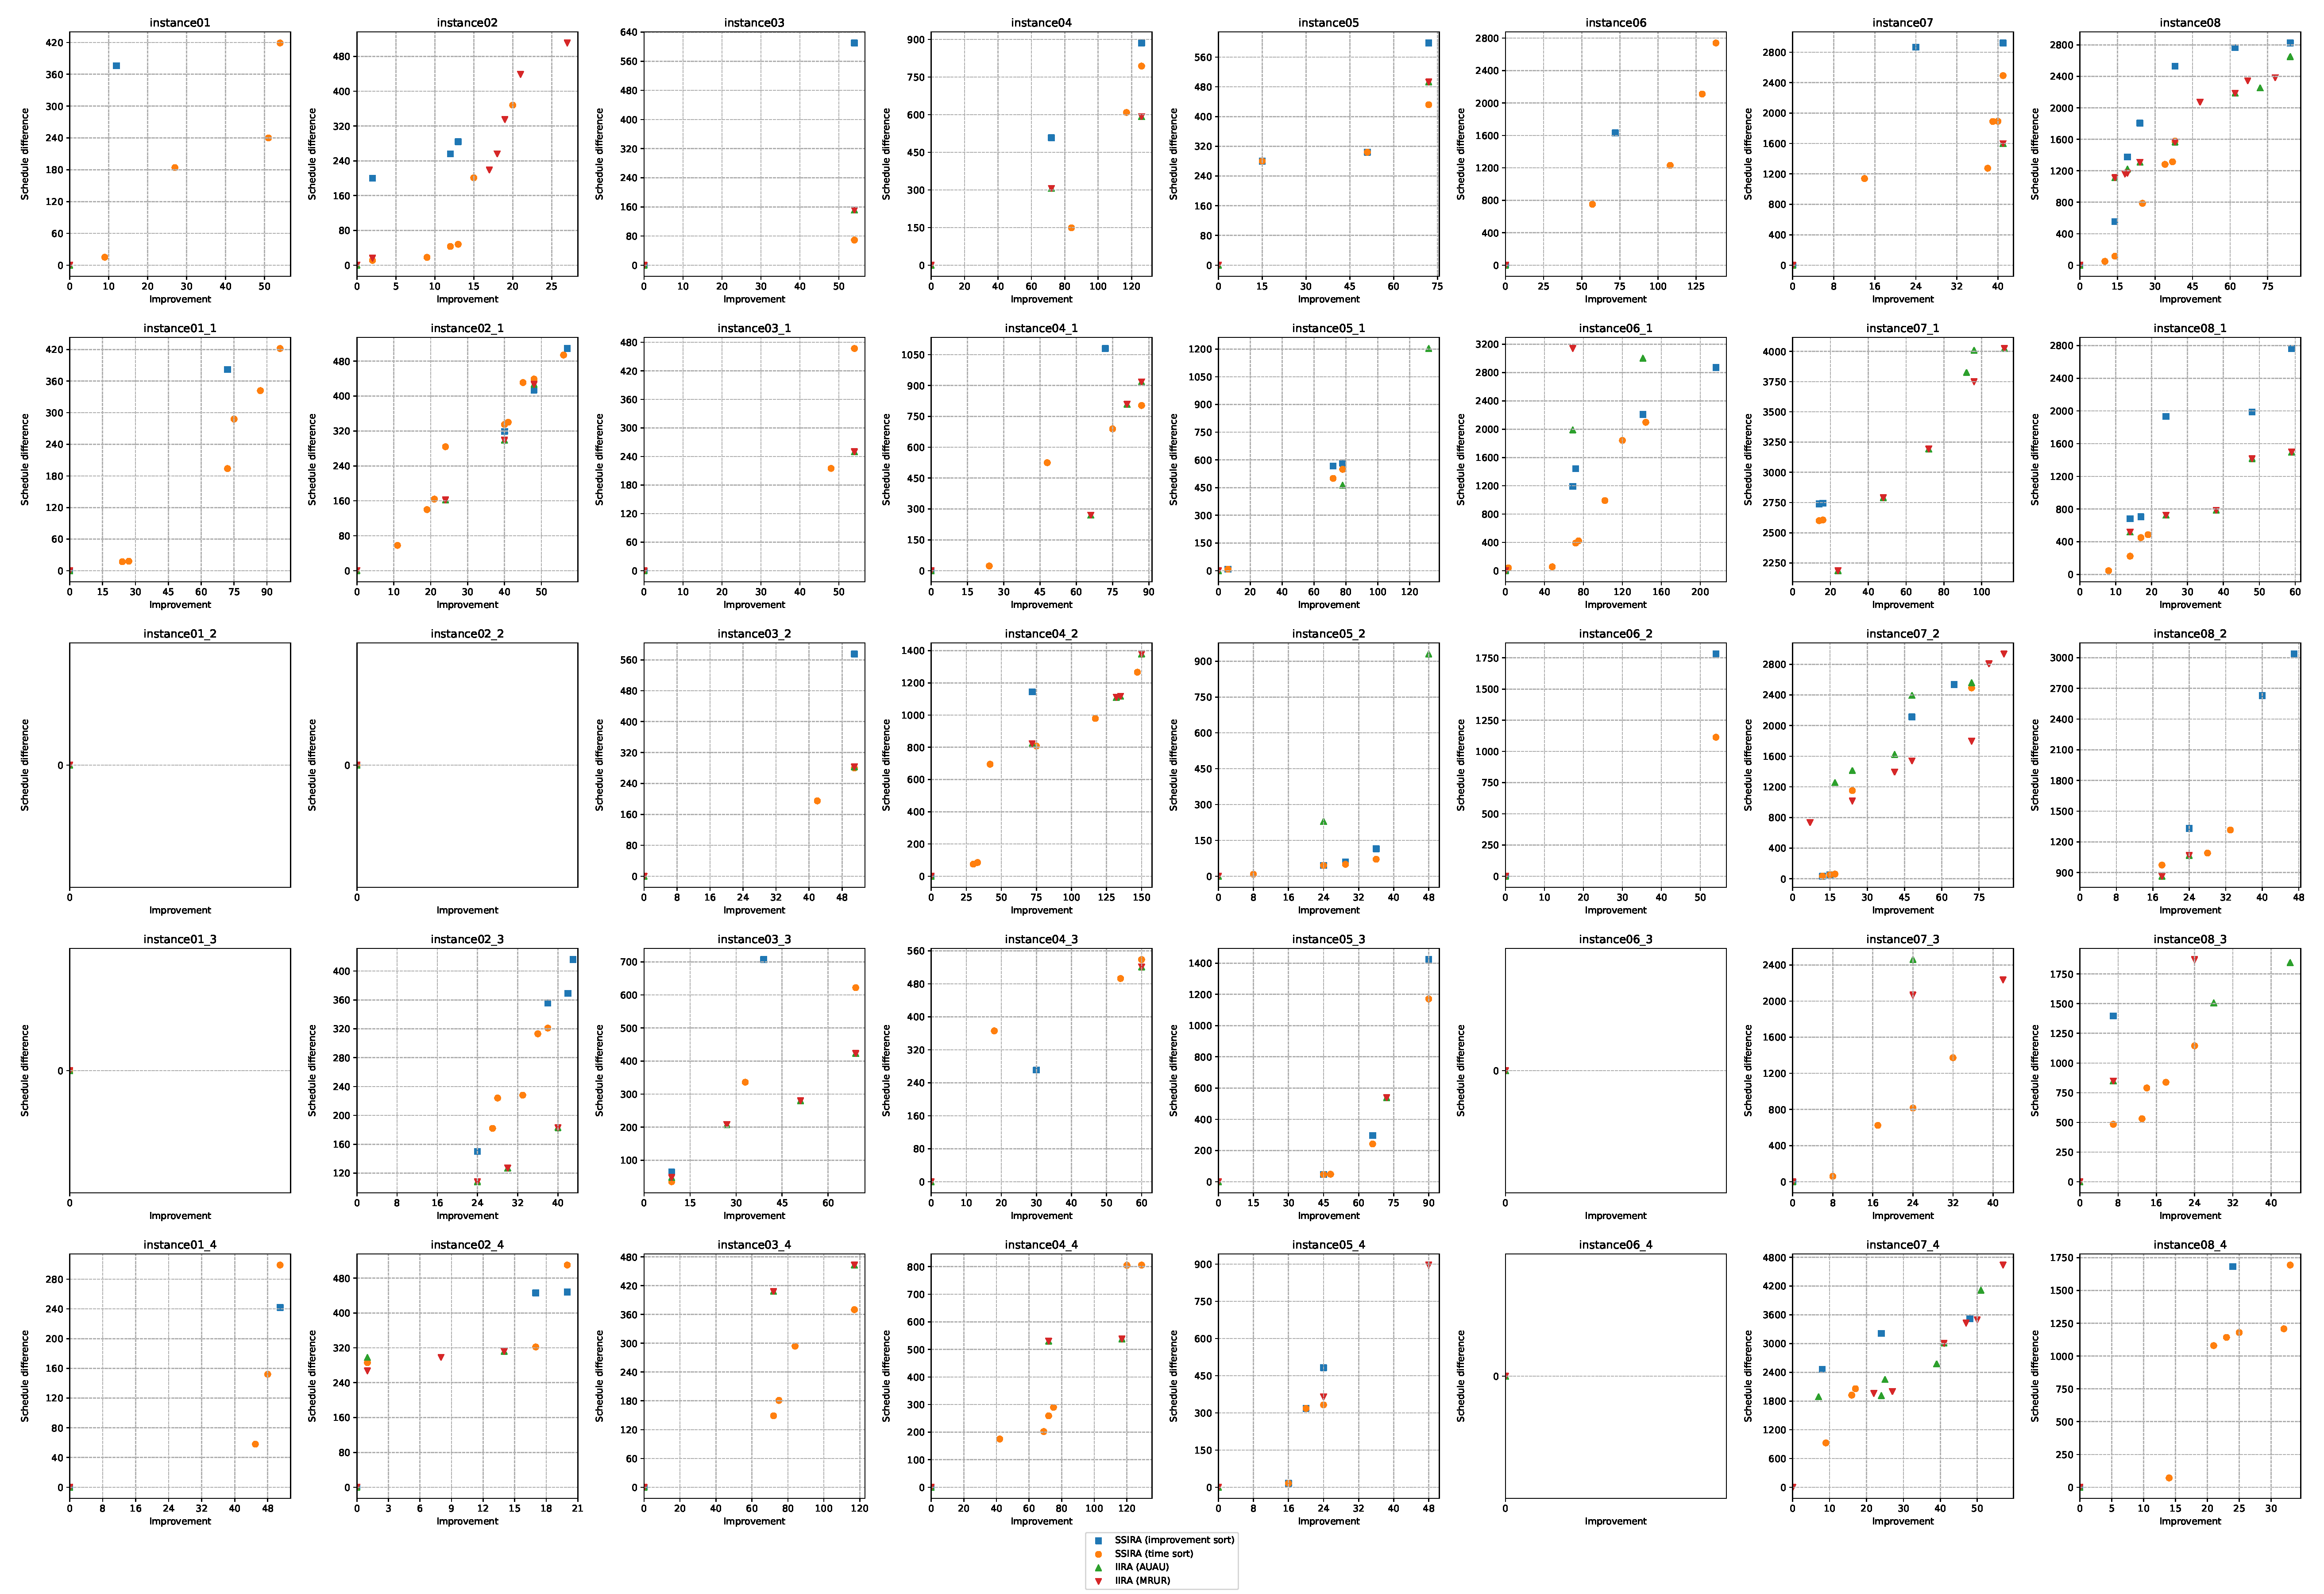
\includegraphics[angle=270,width=\textwidth]{img/exp_improv_diff.pdf}
    \caption{
        Achieved improvement (x-axis) to schedule
        difference (y-axis) for every experiment instance.
        }
    \label{fig:exp-full/improv-diff}
\end{figure}

\begin{figure}[p]
    \centering
    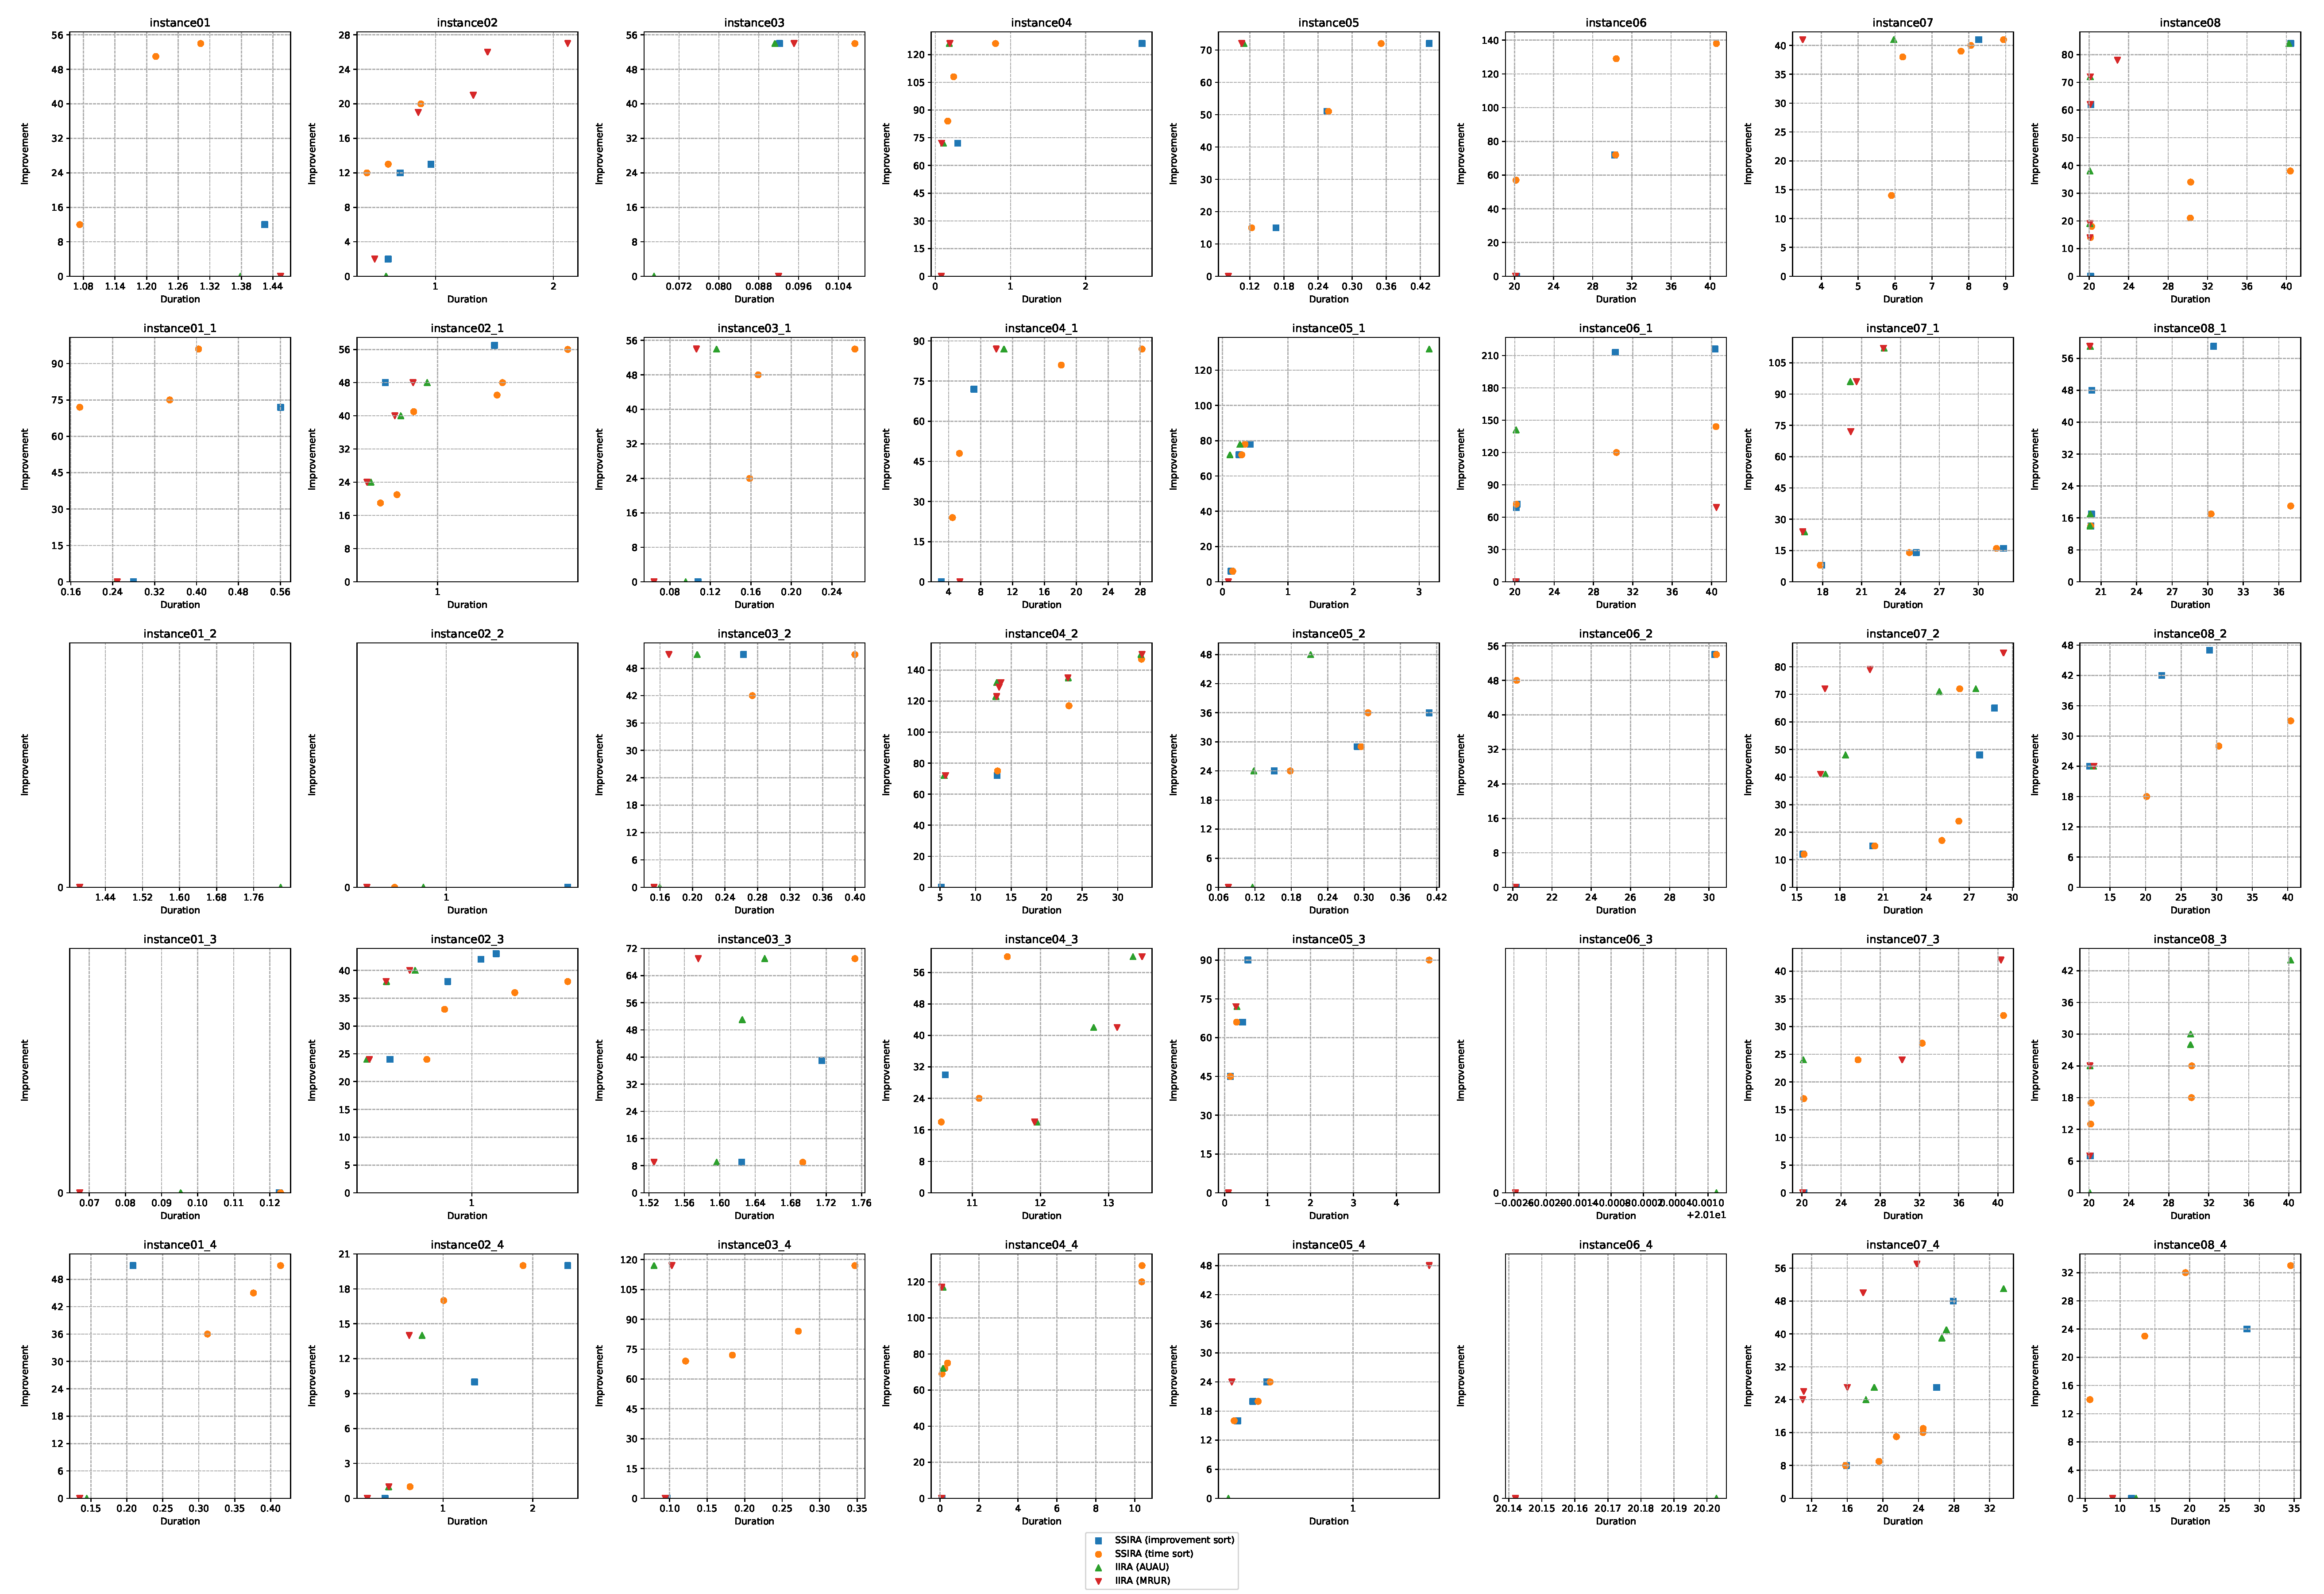
\includegraphics[angle=270,width=\textwidth]{img/exp_duration_improv.pdf}
    \caption{
        Evaluation duration (x-axis) to achieved
        improvement (y-axis) for every experiment instance.
        }
    \label{fig:exp-full/duration-improv}
\end{figure}
